\section{FUNCTIONS, LIMITS, AND CONTINUITY}

\subsection{Scalar and Vector-Valued Functions}

\begin{exercise} \label{e2.1.1}
    Find the parametrizations of each of the following lines:
    \begin{enumerate}
        \item \( 3x_1 + 4x_2 = 6 \)
        
        \item The line with slope \( \frac{1}{3} \) that passes through \( \begin{bmatrix} -1 \\ 2 \end{bmatrix} \)
        
        \item The line through \( A = \begin{bmatrix} 1 \\ 2 \\ 1 \end{bmatrix} \) and \( B = \begin{bmatrix} 2 \\ 1 \\ 0 \end{bmatrix}  \)
        
        \item The line through \( A = \begin{bmatrix} -2 \\ 1 \end{bmatrix} \) perpendicular \( A = \begin{bmatrix} 3 \\ 5 \end{bmatrix}  \)
        
        \item The line through \( \begin{bmatrix} 1 \\ 1 \\ 0 \\ -1 \end{bmatrix} \) parallel to \( \mathbf{g}(t) = \begin{bmatrix} 2+t \\ 1-2t \\ 3t \\ 4-t \end{bmatrix}  \)
    \end{enumerate}
    
    \begin{proof}
        \begin{enumerate}
            \item \[ \mathbf{f}(t) = \begin{bmatrix} t \\ -\frac{3}{4} t + 6 \end{bmatrix} \]
            
            \item \[ \mathbf{f}(t) = t \begin{bmatrix} 1 \\ 3 \end{bmatrix} + \begin{bmatrix} -1 \\ 2 \end{bmatrix} = \begin{bmatrix} t-1 \\ 3t+2 \end{bmatrix} \]
            
            \item \[ \mathbf{f}(t) = t \left( \begin{bmatrix} 1 \\ 2 \\ 1 \end{bmatrix} - \begin{bmatrix} 2 \\ 1 \\ 0 \end{bmatrix} \right) + \begin{bmatrix} 2 \\ 1 \\ 0 \end{bmatrix} \]
            
            \item \[ \mathbf{f}(t) = t \begin{bmatrix} 1 \\ -\frac{3}{5} \end{bmatrix} + \begin{bmatrix} -2 \\ 1 \end{bmatrix} \]
            
            \item \[ \mathbf{g}(t) = \begin{bmatrix} 2+t \\ 1-2t \\ 3t \\ 4-t \end{bmatrix} = t \begin{bmatrix} 1 \\ -2 \\ 3 \\ -1 \end{bmatrix} + \begin{bmatrix} 2 \\ 1 \\ 0 \\4 \end{bmatrix} \]
            Thus
            \[ \mathbf{f}(t) = t \begin{bmatrix} 1 \\ -2 \\ 3 \\ -1 \end{bmatrix} + \begin{bmatrix} 1 \\ 1 \\ 0 \\ -1 \end{bmatrix} \]
        \end{enumerate}
    \end{proof}
\end{exercise}

\begin{exercise} \label{e2.1.2}
    \begin{enumerate}
        \item Give parametric equations for the circle \( x^2 + y^2 = 1 \) in terms of the length \( t \) pictured in the figure.
        
        \item Use your answer to the first part to produce infinitely many positive integer solutions of \( X^2 + Y^2 = Z^2 \) with distinct ratios \( \frac{Y}{X} \)
    \end{enumerate}
    
    \begin{center}
        \begin{tikzpicture}
            \draw[thick] (-1.5,0) -- (1.5,0); % x-axis
            \draw[thick] (0,-1.5) -- (0,1.5); % y-axis
            \draw (0,0) circle(1); % unit circle
            \draw (-1,0) circle(1pt); % line start
            \draw (-1,0) -- (0.6,0.8); % line
            \draw (0.6,0.8) circle(1pt); % line start
            \draw (-1,0) node[anchor=north east] {$\begin{bmatrix} -1 \\ 0  \end{bmatrix}$}; % line start label
            \draw (0.6,0.8) node[anchor=south west] {$\begin{bmatrix} x \\ y  \end{bmatrix}$}; % line end label
            \draw[very thick,red] (0,0) -- (0,0.5); % t length
            \draw[red] (0,0.25) node[anchor=west] {$t$};
            
        \end{tikzpicture}
    \end{center}
    
    \begin{proof}
        \begin{enumerate}
            \item By similar triangles we have that 
            \[ t = \frac{y}{x+1} \]
            which produces the following system:
            \[ \begin{cases} t(x+1) &= y \\ x^2 + y^2 &= 1 \end{cases} \]
            whose solution yields
            \[ \mathbf{f}(t) = \begin{bmatrix} \frac{1-t^2}{1+t^2} \\ \frac{2t}{1+t^2} \end{bmatrix} \]
            
            \item \[ \left\{ \left( 1-t^2, 2t, 1+t^2 \right): t \in \mathbb{Z} \right\} \]
            
            From the figure it is clear that, for \( t > 0 \), \( \frac{Y(t_1)}{X(t_1)} = \frac{Y(t_2)}{X(t_2)} \) iff \( t_1 = t_2 \).
        \end{enumerate}
    \end{proof}
\end{exercise}

\begin{exercise} \label{e2.1.3}
    A string is unwound from a circular reel of radius \( a \), being pulled taut at each instant. Give parametric equations for the tip of the string \( P \) in terms of the angle \( \theta \), as pictured below.
    
    \begin{center}
        \begin{tikzpicture}
            \draw[thick] (-5,0)
            -- (5,0); % x-axis
            
            \draw[thick] (0,-5)
            -- (0,5); % y-axis
            
            \draw (0,0) circle(1);
            
            \draw (0,0)
            -- (-0.354,0.345) node [anchor=east] {$a$}
            -- (-0.707,0.707); % r
            
            \draw (0.2,0) arc (0:135:0.2); % angle
            
            \draw (0.1,0) node [anchor=south west] {$\theta$}; %theta
            
            \draw (-0.707,0.707)
            -- (0.959,2.373);% s
            
            \filldraw (0.959,2.373) circle(1pt);
            
            \draw (0.959,2.373) node [anchor=south west] {$p$}; % label
            
            \draw[domain=0:360,samples=100]
            plot ({cos(\x)+((0.01745 * \x) * sin(\x))},{sin(\x)-((0.01745 * \x)*cos(\x))});
        \end{tikzpicture}
    \end{center}
    
    \begin{proof}
        From the graph we can see that the point \( p \) will be the sum of the radius vector \( r \) and the vector tangent to the circle \( s \). Given that the string is taut, it follows that 
        
        \[ r \cdot s = \begin{bmatrix} x \\ y \end{bmatrix} \cdot \begin{bmatrix} a \cos(\theta) \\ a\sin(\theta) \end{bmatrix} = 0 \]. 
        
        Furthermore, since the string is being unwound, we know that 
        
        \[ \vert \vert s \vert \vert = a \theta \]
        
        Thus, we have the system
        
        \[
        \begin{cases}
            &x\cos(\theta) + y\sin(\theta) = 0 \\
            &x^2 + y^2 = (a\theta)^2
        \end{cases}
        \]
        
        Solving for \( x(\theta) \) and \( y(\theta) \) yields
        
        \[
        \mathbf{f}(\theta) = 
        a \begin{bmatrix} 
            \cos(\theta) + \theta\sin(\theta) \\ 
            \sin(\theta) - \theta cos(\theta) 
        \end{bmatrix}
        \]

        \begin{center}
            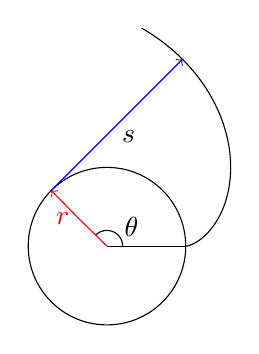
\begin{tikzpicture}
                \draw (0,0)
                -- (1,0);
                
                \draw (0,0) circle(1);
                
                \draw[->,red] (0,0)
                -- (-0.354,0.345) node [anchor=east] {$r$}
                -- (-0.707,0.707); % r
                
                \draw (0.2,0) arc (0:135:0.2); % angle
                
                \draw (0.1,0) node [anchor=south west] {$\theta$}; %theta
                
                \draw[->,blue] (-0.707,0.707)
                -- (0.959,2.373) ;% s
                
                \draw (0.480,1.187) node [anchor=south east] {$s$}; % label
                
                \draw[domain=0:150,samples=100]
                plot ({cos(\x)+((0.01745 * \x) * sin(\x))},{sin(\x)-((0.01745 * \x)*cos(\x))});
            \end{tikzpicture}
        \end{center}
    \end{proof}
\end{exercise}

\subsection{A Bit of Topology in \( \mathbb{R}^n \)}

\subsection{Limits and Continuity}